% Chapter Template

\chapter{Model Development} % Main chapter title

\label{Chapter3} % Change X to a consecutive number; for referencing this chapter elsewhere, use \ref{ChapterX}

\lhead{Chapter 3. \emph{Model Development}} % Change X to a consecutive number; this is for the header on each page - perhaps a shortened title

%----------------------------------------------------------------------------------------
%	SECTION 1
%----------------------------------------------------------------------------------------

\section{Finite Element Modeling Framework}
%-----------------------------------
%	SUBSECTION 1
%-----------------------------------
\subsection{Microstructure Instantiation}
We have used an in-house MATLAB code to instantiate the 2D microstructures of a dual-phase (DP) steel comprising of ferrite and martensite phases. This code employs a weighted Voronoi tessellation algorithm for random positioning of grain centers within the simulation domain. The grain size distribution and volume fractions of the respective phrases are pre-defined based on experimental measurements. Figure-\ref{fig:grain-trans} shows the grain map of the microstructure generated by this algorithm. The desired mean radius $r_i$ and  volume fractions $V_i$ are given as inputs to the algorithm. The number of grains are calculated by the algorithm as $(Area\times V_i)/(\pi r_i^2)$. The sizes of these $n_i$ grains are generated randomly. The subscript $i$ has a value of 1 for ferrite and 2 for martensite. Details of the microstructure instantiation algorithm are given in Ref.  \cite{patra2015modeling}. The Trelis meshing software has been used to mesh the 2D microstructure with voxel-based elements. An element size of $0.25 \mu m$ is used to mesh the simulation domain of $100\times100 \mu m^2$.
\begin{figure}[!h]
	\centering
	\includegraphics[width=0.65\textwidth]{Pictures/grain-trans.png}
	\hspace{1mm}
	\caption{Grain Map (colours are random and only to demarcate one grain from another)} 
	\label{fig:grain-trans}
\end{figure}
%-----------------------------------
%	SUBSECTION 2
%-----------------------------------
\subsection{Constitutive Model}
We have used a J2 plasticity constitutive modeling framework for the finite element (FE) computations. This framework is based on a finite deformation, dislocation density based model adapted from a crystal plasticity model previously used to model deformation behavior of various metallic systems \cite{POKHAREL2019201} \cite{THOOL2020102785}. While this is not a new feature of this work, details are provided here for completeness. 

In this framework, the deformation gradient is multiplicatively decomposed into the elastic and plastic parts: 
\begin{equation}
\boldsymbol{F} = \boldsymbol{F^e} \cdot \boldsymbol{F^p}
\end{equation}
where, $\boldsymbol{F^p}$ relates the reference configuration to an intermediate configuration and accounts for shear due to plastic deformation, while $\boldsymbol{F^e}$ relates the intermediate configuration to the current, deformed deformation and accounts for the rigid body rotation and elastic distortion. 
The elastic Green strain is given as:
\begin{equation}
\boldsymbol{E^e} = \frac{1}{2} (\boldsymbol{F^e}^T \cdot \boldsymbol{F^e} - \boldsymbol{I})
\end{equation}
Further, the second Piola-Kirchoff tensor is related to the elastic Green strain via the fourth rank elasticity tensor $\boldsymbol{C_o}$, i.e.,
\begin{equation}
    \boldsymbol{\sigma^{PK2}} = \boldsymbol{C_o} : \boldsymbol{E^e}
\end{equation}
The second Piola-Kirchoff tensor $\boldsymbol{\sigma^{PK2}}$ and the cauchy stress $\boldsymbol{\sigma}$
\begin{equation}
    \boldsymbol{\sigma} = \frac{\boldsymbol{F^e} \cdot \boldsymbol{\sigma^{PK2}} \cdot \left (\boldsymbol{F^e}\right)^T}{det\left (\boldsymbol{F^e}\right)}
\end{equation}
The von Mises effective stress, $\bar{\sigma}$ can be given in terms of the deviatoric part $\boldsymbol{S}$ of the Cauchy stress, i.e.,
\begin{equation}
    \boldsymbol{S} = dev(\boldsymbol(\sigma)) = \boldsymbol{\sigma} - \frac{\left (tr(\boldsymbol{\sigma}) \right )\boldsymbol{I}}{3}
\end{equation}
\begin{equation}
    \bar{\sigma} = \sqrt{\frac{3}{2}\boldsymbol{S}:\boldsymbol{S}}
\end{equation}
In J2 plasticity, the equivalent plastic strain rate $\dot{\bar{\epsilon}}^p$ is given as a function of the von Mises effective stress $\bar{\sigma}$. In this finite deformation framework, the plastic deformation gradient is related to the plastic velocity gradient as: $\boldsymbol{\dot{F}^p} = \boldsymbol{L^p} \cdot \boldsymbol{F^p}$, where $\boldsymbol{L^p}$ is the velocity gradient given by:
\begin{equation}
    \boldsymbol{L^p} = \dot{\bar{\epsilon}}^p \cdot \boldsymbol{N^p}
\end{equation}
where $\dot{\bar{\epsilon}}^p$ is the effective plastic strain, and $\boldsymbol{N^p}$ gives the direction of the plastic flow given by:
\begin{equation}
   \boldsymbol{N^p} =  \sqrt{\frac{3}{2}}\frac{\boldsymbol{S}}{\bar{\sigma}}
\end{equation}
The equivalent plastic strain rate is modelled using a Kocks-type activation enthalpy-driven flow rule:
\begin{equation}
\dot{\bar{\epsilon}}^p = \dot{\bar{\epsilon}}^p_o\exp\left(\frac{-\Delta F_g}{kT}\left(1 - \left(\frac{\sigma_{eff} - S_a}{S_t}\right)^p\right)^q\right)
\end{equation}
where, $\Delta F_g$ is the activation energy for dislocation glide, $S_a$ is athermal slip resistance, and $S_t$ is the thermal slip resistance, $p$ and $q$ are parameters used to model the shape of the activation enthalpy curve. The athermal slip resistance $S_a$ can be given by:
\begin{equation}
    S_a = \frac{h_p}{\sqrt{d}} + Gb\sqrt{q_p\rho}
\end{equation}
where, $h_p$ is the Hall-Petch hardening constant, $d$ is the grain size, $G$ is the shear modulus, $b$ is the Burgers vector, $q_p$ is the dislocation barrier strength and $\rho$ is the total dislocation density. $\rho$ is defined as the sum of immobile ($\rho_M)$ and mobile ($\rho_I)$ dislocation densities, i.e., 
\begin{equation}
    \rho = \rho_M + \rho_I
\end{equation}
The evolution of the dislocation densities with respect to time depends on the equivalent tensile plastic strain rate as:
\begin{equation}
\dot{\rho_M} = \frac{k_mul}{b}\sqrt{\Sigma\rho}|\dot{\bar{\epsilon}}^p| - \frac{2R_c}{b}\rho_M|\dot{\bar{\epsilon}}^p| - \frac{1}{b\lambda}|\dot{\bar{\epsilon}}^p|
\end{equation}
\begin{equation}
\dot{\rho_I} = \frac{1}{b\lambda}|\dot{\bar{\epsilon}}^p| - k_{dyn}\rho_I|\dot{\bar{\epsilon}}^p|
\end{equation}
where $\lambda = \frac{1}{\beta\sqrt{\rho}}$ is effective mean free path, $\beta$ is a constant associated with dislocation trapping, $k_{mul}$ is the dislocation multiplication rate constant and $R_c$ is the critical capture radius. The first term in Eq. 3.12 represents the multiplication of mobile dislocations at existing dislocations, while the second term represents the mutual annihilation of dislocation dipoles, and third term is the trapping of mobile dislocations at barriers. $k_{dyn}$ is the material constant associated with dynamic recovery of immobile dislocations due to thermally activated processes. The first term in Eq. 3.13 represents the rate at which mobile dislocations are trapped in barriers and become immobile, while the second term is the rate at which the immobile dislocations are annihilated due to dynamic recovery.

The constitutive model has been implemented as material model and interfaced with the open source finite element code, MOOSE \cite{permann2020moose}. The individual phases have been calibrated to the response of the ferrite and martensite phases based on available data in the literature. Further details and model parameters are given in Basu et al \cite{soudip}.

\subsection{Loading And Boundary Conditions}
A mesh size of $0.25 \mu m$ is used with a simulation domain size of $100\times100 \mu m^2$. The simulation domain has 40,000 elements.A generalized plane strain assumption is used in these essentially 2D simulations. The bottom face of the simulation domain is constrained in the y-direction, while the left face is constrained in the x-direction to resemble an axisymmetric model. The corner node common to both these faces is fully constrained to prevent rigid body motion. Displacement-controlled tensile loading is applied on the top face at a strain rate of $5\times10^{-3}s^{-1}$.
\begin{figure}[!h]
	\centering
	\includegraphics[width=\textwidth]{Pictures/result-fe.png}
	\hspace{1mm}
	\caption{Contour of (a) Effective Strain (b) Triaxiality (c) Vonmises Stress at the last time step} 
	\label{fig:exo-plots}
\end{figure}
\begin{figure}[!h]
	\centering
	\includegraphics[width=0.8\textwidth]{Pictures/stress-strain.eps}
	\hspace{1mm}
	\caption{Effective strain vs Vonmises stress curve} 
	\label{fig:stress-strain}
\end{figure}

\section{Data Extraction from FE Results}
The simulation results of the FE model are output to an EXODUS data file. The EXODUS format is a binary file which is used for FE pre- and post-processing. Data used to define the finite element mesh, along with both the boundary conditions and load application points are includes in the file. The EXODUS format is advantageous as it combines the mesh data as well as the results data in a single file. This assures the user that the results are consistent with the model \cite{mills1988exodus}. However, to access this data in a usable and easily interpretable way, special software are used. For the purpose of this project, we have used the  Sandia Engineering Analysis Code Access System (SEACAS) developed by Sjaardema \cite{seacas}. The library consists of packages which can convert an EXODUS file's data to different formats like text file and MATLAB data files. The Python package has been used for this project which makes reading the data from an EXODUS file viable through a python script. The package provides a number of predefined functions to extract different information from the EXODUS file. Using these functions, we have extracted all the data from the EXODUS file to a csv format. The csv format has all the element variable values at every time-step for every element. The script is written in Python 2.7.17 and take approximately 10 minutes to execute. The time taken by the script varies with the mesh size and number of variables in the exodus file.   

\section{Machine Learning Framework}
\subsection{ANN Model}
At the basic level, the process of developing an ANN model (or any learning model) has two primary steps. First one being, selecting the relevant, representative and compact set of  features and then developing a relation between them to get the desired result. Elimination of irrelevant features and selection or relevant ones is one of the central tasks in machine learning \cite{blum1997selection}. In this context, it has been assumed that the observed heterogeneity in deformation is due to the underlying heterogeneity of the microstructure. The features of interest are highlighted in the Table \ref{tab:feature-table}. 
\begin{table}
\begin{center}
\begin{tabular}{|c|c|}
\hline
Feature & Description \\
\hline
\textit{x} & x-coordinate of the element \\
\hline
\textit{y} & y-coordinate of the element \\
\hline
\textit{p} & Phase to which the element belongs (ferrite or martensite) \\
\hline
\begin{math}{\epsilon_{app}}\end{math}& Applied (or nominal) strain \\
\hline
\end{tabular}
\end{center}
\caption{\label{tab:feature-table}Selected feature names and descriptions.}
\end{table}

The output variables of interest are effective strain, ${\bar{\epsilon}}$, von Mises effective stress, $\bar{\sigma}$, and stress triaxiality ratio. While, effective strain and effective stress can be correlated with plastic deformation in the respective phases, the stress triaxiality ratio (given as the ratio of the mean stress over the von Mises effective stress) provides a measure of the development of multi-axial stress states that may contribute to eventual failure initiation in the material. In the present context, the ferrite-martensite interfaces are potential sites for failure initiation in DP steels and hence it is pertinent to be able to predict the stress triaxiality ratio as well. For each element, ${\bar{\epsilon}}$, $\bar{\sigma}$ and triaxiality ratio are recorded at applied strain intervals of $0.01$. The simulation is run up to $0.15$ nominal strain, thus providing us a total of fifteen datasets at $0.01$ nominal strain intervals. The mesh consists of $400\times400$ elements, making the length of every feature and target variable vector $2,400,000$. Thus, the shape of our input is $2,400,000\times4$ and the corresponding shape of output is $2,400,000\times3$. 

Note that feature selection depends on the output variables of interest and may vary if it is desired to output a different set of variables. Mangal and Holm \cite{MANGAL2018122} provide a detailed study of the performance of neural network models with different input features for a crystal plasticity model. In the context of a J2 plasticity model, we assume the features given in Table \ref{tab:feature-table} to be the most relevant for the present problem.

Any ANN model is very sensitive to the magnitude of the training data. Given that we are interested in strains and stresses, whose magnitudes are generally many orders apart, all the data has been normalized within the range $[0,1]$ in the present work. The normalised values $x_i^n$ for any training variable $x_i$ are calculated as:
\begin{equation}
    x_i^n = \frac{x_i - x_{min}}{x_{max} - x_{min}}
\end{equation}
In this work, the mean-squared error function (MSE) has been used and the sigmoid function has been employed as the activation function for every neuron. The completed training and model development process has been performed using python and Keras with a Tensorflow backend. Data splitting is another important task during data splitting where hold-out validation is employed to ensure generalisation \cite{may2010data}. The dataset is split into training ($80\%$) and testing ($20\%$) datasets. The training data is used to for training and learning of the ANN, whereas the testing dataset is used to check the accuracy of the fitted parameters. The validation dataset is unseen by the ANN model, therefore predictions made by the model on the validation dataset represents the degree to which the model generalizes over our data. A number of networks were trained on this data with different architectures. The network which performed relatively better than others consisted of 4 inputs, 3 hidden layers and 3 outputs. The training of the neural network is performed over 5 epochs and takes 106 minutes to train. 
\begin{figure}[!h]
	\centering
	\includegraphics[width=0.9\textwidth]{Pictures/my-ann.png}
	\hspace{1mm}
	\caption{Schematic of proposed ANN architecture} 
	\label{fig:my-ann}
\end{figure}
\begin{figure}[!h]
	\centering
	\includegraphics[width=0.8\textwidth]{Pictures/training_process.eps}
	\hspace{1mm}
	\caption{Learning curve showing the evolution of MSE loss over training data-set} 
	\label{fig:ann-training}
\end{figure}

\subsection{LSTM Model}
LSTMs have shown great accuracy in predicting sequence and time series data. The evolution of local strain distribution can be formulated as a sequence modeling problem. As with ANN, we are focusing on three output variables in our model, namely, effective strain, ${\bar{\epsilon}}$, von Mises effective stress,  $\bar{\sigma}$, and stress triaxiality ratio. For every element, the values of these variables are recorded for every $0.01$ nominal strain interval. As mentioned previously, the simulation is run till $0.15$ nominal strain and hence our data contains $15$ strain steps. Each element is associated with 3 sequences of length 15, and as there are $400\times400$ elements the total number of series or model predicts is $400\times400\times3$. For a given strain step $t$, $400\times400\times3$ length vector $\boldsymbol{X_t}$ is input to the LSTM model and used to predict the output vector, $\boldsymbol{Y_t}$ which consists of values at the next strain step in the series $X_{t+1}$. The structure of the data can be understood better through the Table \ref{tab:lstm-data-table}. All data was normalized within the range of $[0,1]$. The data was split into training ($70\%$) and test ($30\%$) datasets, meaning the training dataset consisted of only the first $10$ strain steps. The model was trained using the training dataset run over 300 epochs. The last $5$ strain steps were used to check how well the model performs on data it has not seen before. The model consists of $8$ LSTM layers with $200$ neurons in each layer. The activation function employed in this case is ReLU. The choice of activation function is driven by the reduction in MSE over the epochs. Figure \ref{fig:diff-activation-lstm} shows the performance of different activation functions while training the same dataset. The number of layers and neuron are the same for these model, only the variation with activation function is checked for. It can be observed that ReLU performs better than the other two activation functions by at least two orders of magnitude of MSE.

\begin{table}
\begin{center}
\begin{tabular}{|c|c|}
\hline
Input (\begin{math}\boldsymbol{X}\end{math})&Output (\begin{math}\boldsymbol{Y}\end{math}) \\
\hline
\begin{math}\boldsymbol{X_1}\end{math}& \begin{math}\boldsymbol{X_2}\end{math} \\
\begin{math}\boldsymbol{X_2}\end{math}& \begin{math}\boldsymbol{X_3}\end{math}  \\
\begin{math}\boldsymbol{X_3}\end{math}& \begin{math}\boldsymbol{X_4}\end{math} \\
. & . \\
. & . \\
. & . \\
. & . \\
\begin{math}\boldsymbol{X_{10}}\end{math}& \begin{math}\boldsymbol{X_{11}}\end{math} \\
\hline
\end{tabular}
\end{center}
\caption{\label{tab:lstm-data-table}Training data format for LSTM.}
\end{table}

\begin{figure}[!h]
	\centering
	\includegraphics[width=0.7\textwidth]{Pictures/lstm-res/lstm-tanh_loss.eps}
	\hspace{1mm}
	\caption{Learning curve showing the evolution of MSE loss over training data-set.} 
	\label{fig:ann-training}
\end{figure}

\begin{figure}[!h]
	\centering
	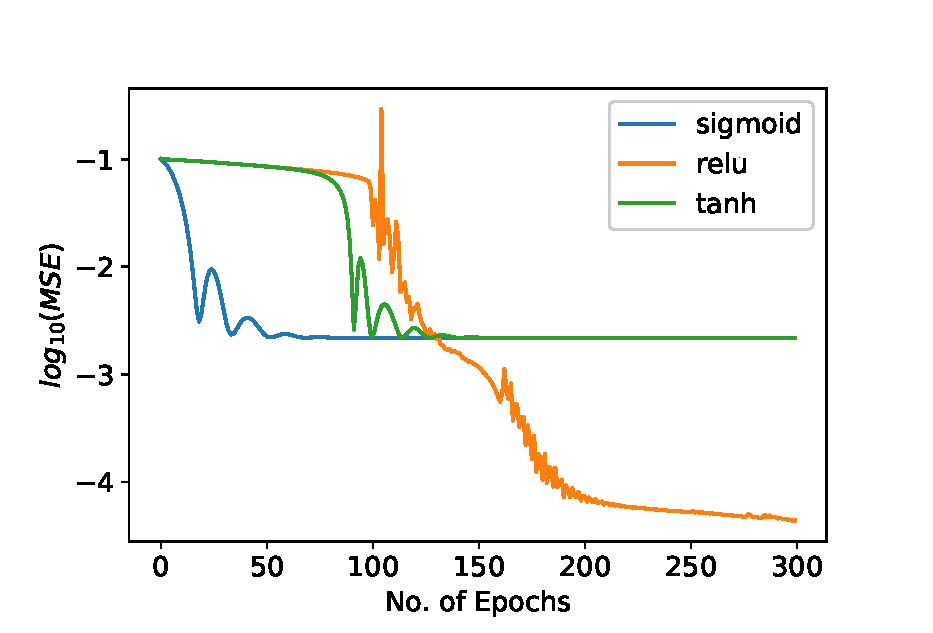
\includegraphics[width=0.7\textwidth]{Pictures/lstm-res/lstm-sctivations_log.eps}
	\hspace{1mm}
	\caption{Comparative study of MSE obtained in training models with different activation functions} 
	\label{fig:diff-activation-lstm}
\end{figure}
\begin{sidewaysfigure}[ht]
	\includegraphics[width=0.95\textwidth]{Pictures/lstm-res/flow-purple.png}
	\hspace{1mm}
	\caption{Schematic representation of the proposed ML framework} 
	\label{fig:flow-chart}
\end{sidewaysfigure}
\iffalse
Along with a vanilla LSTM, two modification of LSTMs were also trained:
\begin{enumerate}
\item \textbf{Auto-regressive}: The training of procedure of this LSTM is similar to that of a vanilla LSTM, however the difference arises in the way predictions are made. For a regular LSTM, to predict the value of a sequence at time $t$ one would need to know all the true values till time $t-1$ and so on for $t+1$. In an auto-regressive methodology once an initial prediction is made using the available sequence data, all further predictions are made using this initial prediction. Say for example, a prediction is made for time $t$. To predict $t+1$ time-step, instead of using the input sequence data we use this predicted value at time $t$. This enables our LSTM to predict sequence values further into the future without requiring input data up to the penultimate step.
\item \textbf{LSTM-FC}: This kind of model consists two major components: (1) A long-short term memory based temporal simulator to model the local strain developments and (2) A neural network to capture the spatial dependencies of strain between a central element and it's neighbours. The LSTM capable of handling long term dependencies handles only the temporal information in the data, and the spatial information is incorporated using a fully connected neural network. The neural network is trained such that given 8 neighbouring elements' property values it can make predictions  for the central element. 
\end{enumerate}
\fi